%
% This is a borrowed LaTeX template file for lecture notes for CS267,
% Applications of Parallel Computing, UCBerkeley EECS Department.
% Now being used for CMU's 10725 Fall 2012 Optimization course
% taught by Geoff Gordon and Ryan Tibshirani.  When preparing
% LaTeX notes for this class, please use this template.
%
% To familiarize yourself with this template, the body contains
% some examples of its use.  Look them over.  Then you can
% run LaTeX on this file.  After you have LaTeXed this file then
% you can look over the result either by printing it out with
% dvips or using xdvi. "pdflatex template.tex" should also work.
%

\documentclass[UTF8,oneside]{article}

% \usepackage[UTF8,scheme=plain]{ctex}
\usepackage[AutoFakeBold,AutoFakeSlant,CJKecglue]{xeCJK}  % 载入 xeCJK以支持中文,支持伪粗体,伪斜体 , 去掉CJK 文字与西文字体间的空格
\usepackage[margin=1in]{geometry}
\usepackage{amsmath,amsthm,amssymb}
\usepackage{graphicx}
\usepackage{autobreak}
\usepackage{tikz}
\usetikzlibrary{positioning} %为了实现相对位置的设定
\usepackage{xcolor} %为了实现不同的颜色
\setCJKmainfont{宋体}                                         % 设置中文中文字体
\setCJKmonofont{宋体}                                        % 设置中文等宽字体
% \setCJKsansfont{宋体}
% \setCJKmainfont{SimSun}[BoldFont=SimHei, ItalicFont=KaiTi]
\setlength{\oddsidemargin}{0.25 in}
\setlength{\evensidemargin}{-0.25 in}
\setlength{\topmargin}{-0.6 in}
\setlength{\textwidth}{6.5 in}
\setlength{\textheight}{8.5 in}
\setlength{\headsep}{0.75 in}
\setlength{\parindent}{0 in}
\setlength{\parskip}{0.1 in}

%
% ADD PACKAGES here:
%

\usepackage{amsmath,amsfonts,graphicx}

%
% The following commands set up the lecnum (lecture number)
% counter and make various numbering schemes work relative
% to the lecture number.
%
\newcounter{lecnum}
\renewcommand{\thepage}{\thelecnum-\arabic{page}}
\renewcommand{\thesection}{\thelecnum.\arabic{section}}
\renewcommand{\theequation}{\thelecnum.\arabic{equation}}
\renewcommand{\thefigure}{\thelecnum.\arabic{figure}}
\renewcommand{\thetable}{\thelecnum.\arabic{table}}

%
% The following macro is used to generate the header.
%
\newcommand{\lecture}[4]{
   \pagestyle{myheadings}
   \thispagestyle{plain}
   \newpage
   \setcounter{lecnum}{#1}
   \setcounter{page}{1}
   \noindent
   \begin{center}
   \framebox{
      \vbox{\vspace{2mm}
    \hbox to 6.28in { {\bf Fundamentals Of Information Science
	\hfill 2022 Spring} }
       \vspace{4mm}
       \hbox to 6.28in { {\Large \hfill Homework4  \hfill} }
       \vspace{2mm}
       \hbox to 6.28in { {\it 学生: #3 \hfill 时间: #4} }
      \vspace{2mm}}
   }
   \end{center}
   \markboth{Lecture #1: #2}{Lecture #1: #2}

}
%
% Convention for citations is authors' initials followed by the year.
% For example, to cite a paper by Leighton and Maggs you would type
% \cite{LM89}, and to cite a paper by Strassen you would type \cite{S69}.
% (To avoid bibliography problems, for now we redefine the \cite command.)
% Also commands that create a suitable format for the reference list.
\renewcommand{\cite}[1]{[#1]}
\def\beginrefs{\begin{list}%
        {[\arabic{equation}]}{\usecounter{equation}
         \setlength{\leftmargin}{2.0truecm}\setlength{\labelsep}{0.4truecm}%
         \setlength{\labelwidth}{1.6truecm}}}
\def\endrefs{\end{list}}
\def\bibentry#1{\item[\hbox{[#1]}]}

%Use this command for a figure; it puts a figure in wherever you want it.
%usage: \fig{NUMBER}{SPACE-IN-INCHES}{CAPTION}
\newcommand{\fig}[3]{
			\vspace{#2}
			\begin{center}
			Figure \thelecnum.#1:~#3
			\end{center}
	}
% Use these for theorems, lemmas, proofs, etc.
\usepackage{amsthm}
\newtheorem*{Solution}{Solution}
\newtheorem{theorem}{Theorem}[lecnum]
\newtheorem{lemma}[theorem]{Lemma}

\newtheorem{proposition}[theorem]{Proposition}
\newtheorem{claim}[theorem]{Claim}
\newtheorem{corollary}[theorem]{Corollary}
\newtheorem{definition}[theorem]{Definition}
% \newenvironment{proof}{{\bf Proof:}}{\hfill\rule{2mm}{2mm}}

% **** IF YOU WANT TO DEFINE ADDITIONAL MACROS FOR YOURSELF, PUT THEM HERE:

\newcommand\E{\mathbb{E}}

\begin{document}
%FILL IN THE RIGHT INFO.
%\lecture{**LECTURE-NUMBER**}{**DATE**}{**LECTURER**}{**SCRIBE**}
\lecture{1}{信息与比特}{华园(202000120027))}{2022.3.17}
%\footnotetext{These notes are partially based on those of Nigel Mansell.}

% **** YOUR NOTES GO HERE:

% Some general latex examples and examples making use of the
% macros follow.
%**** IN GENERAL, BE BRIEF. LONG SCRIBE NOTES, NO MATTER HOW WELL WRITTEN,
%**** ARE NEVER READ BY ANYBODY.

\section*{Problem 1.} % Don't be this informal in your notes!
Run-length encoding
Run-length encoding is a popular variable-length lossless compressor used in fax machines,
image compression, etc. Consider compression of $S^n$- an i.i.d. binary source with very small 1/64 of being 1 using run-length encoding f: A chunk of consecutive r <=127 zeros (resp.
ones) is encoded into a zero (resp. one) followed by an 7-bit binary encoding of r (If there are > 127 consecutive zeros then two or more 8-bit blocks will be output). Compute the average achieved compression rate
$$\lim _{n \rightarrow \infty} \frac{1}{n} \mathbb{E}\left[l\left(f\left(S^{n}\right)\right)\right]$$
How does it compare with the optimal lossless compressor?
\begin{Solution}
\end{Solution}
\begin{table}[h]
\centering
\begin{tabular}{|c|c|c|c|c|}
\hline
$S^n $&$ f(S^n)$&P&Length&normalize\\
\hline
0 & 0000 0001&$\frac{63}{64}*\frac{1}{64}$&8&8\\
\hline
1 & 1000 0001&$\frac{1}{64}*\frac{63}{64}$&8&8\\
\hline
00 &0000 0010&$(\frac{63}{64})^2*\frac{1}{64}$&8&4\\
\hline
11& 1000 0010&$(\frac{1}{64})^2 *\frac{63}{64}$&8&4\\
\hline
... & ...&...&...&...\\
\hline
00000..(127)& 0111 1111&$(\frac{63}{64})^{127}$&8&8/127\\
\hline
11111..(127)& 1111 1111&$(\frac{1}{64})^{127 }$&8&8/127\\
\hline
000000...(k)&....&$(\frac{63}{64})^k$&$(\lfloor \frac{k}{127}+1 \rfloor)*8$&...\\
\hline
111111...(k)&....&$(\frac{1}{64})^k$&$(\lfloor \frac{k}{127}+1 \rfloor)*8$&...\\
\hline
\end{tabular}
\label{TAB1}
\end{table}

\begin{equation}
\begin{aligned}
\lim _{n \rightarrow \infty} \frac{1}{n} E\left[l\left(f\left(S^{n}\right)\right)\right] &=\lim _{n \rightarrow \infty} \frac{1}{n}\left(\frac{63}{64^{2}} \cdot 8 n+\frac{1}{64^{2}} \cdot 8 n+\frac{63^{2}}{64^{3}}+4 n+\frac{63}{64^{3}} \cdot 4 n+\ldots+\left(\frac{63}{64}\right)^{127} \cdot \frac{8 n}{127}+\left(\frac{1}{64}\right)^{127} \cdot \frac{8 n}{127}\right) \\
&=\sum\nolimits_{k=1}^{126}\left[\frac{1}{64} \cdot\left(\frac{63}{64}\right)^{k} \cdot \frac{8}{k}+\frac{63}{64} \cdot\left(\frac{1}{64}\right)^{k} \cdot \frac{8}{k}\right]+\left(\frac{63}{64}\right)^{127} \cdot \frac{8}{127}+\left(\frac{1}{64}\right)^{127} \cdot \frac{8}{127}\\
&\approx 0.646
\end{aligned}
\end{equation}
program:\\
a=0\\
\quad for i in range(1,127):\\
\qquad    m=(1/64)*(63/64)**i*(8/i)+(63/64)*(1/64)**i*(8/i)\\
\qquad    a=a+m\\
a=a+(63/64)**127*(8/127)+(1/64)**127*(8/127)\\
print(a)\#0.6462243257022445\\
because $\delta_n$  is an i.i.d. binary source,so the entropy:\\
\begin{align*}
H(X) &=-n\sum_{n=1}^\infty p(x)log_{2}p(x) \\
&=-n(\frac{1}{64}log_{2}\frac{1}{64}+\frac{63}{64}log_{2}\frac{63}{64})\\
&=0.116n\\
\\
if\;0.116n<L&=0.646n<0.116n+1\\
so\;n&<2\\
\end{align*}
Therefore, we can know that the overall performance of run length coding is worse than the optimal code.

\section*{Problem 2.} % Don't be this informal in your notes!
Find the binary Huffman code for the source with probabilities (1/3,1/5,1/5,2/15,2/15). Argue that this code is also optimal for the source with probabilities ( 1/5 ,1/5,1/5, 1/5,1/5).
\begin{Solution}
\end{Solution}
for probabilities (1/3,1/5,1/5,2/15,2/15).
\begin{center}
  \begin{tikzpicture}
\filldraw [black] (0,1.5) circle (0pt)--node[right=4pt,fill=white]{$1/3$}(0,1.5);
\filldraw [black] (0,0) circle (0pt)--node[right=4pt,fill=white]{$4/15$}(0,0);
\filldraw [black] (0,-1.5) circle (0pt)--node[right=4pt,fill=white]{$1/5$}(0,-1.5);
\filldraw [black] (0,-3) circle (0pt)--node[right=4pt,fill=white]{$1/5$}(0,-3);

\filldraw [black] (3,1.5) circle (0pt)--node[right=4pt,fill=white]{$2/5$}(3,1.5);
\filldraw [black] (3,0) circle (0pt)--node[right=4pt,fill=white]{$1/3$}(3,0);
\filldraw [black] (3,-1.5) circle (0pt)--node[right=4pt,fill=white]{$4/15$}(3,-1.5);

\filldraw [black] (6,1.5) circle (0pt)--node[right=4pt,fill=white]{$3/5$}(6,1.5);
\filldraw [black] (6,0) circle (0pt)--node[right=4pt,fill=white]{$2/5$}(6,0);

\filldraw [black] (-3,1.5) circle (0pt)--node[right=4pt,fill=white]{$1/3$}(-3,1.5);
\filldraw [black] (-3,0) circle (0pt)--node[right=4pt,fill=white]{$1/5$}(-3,0);
\filldraw [black] (-3,-1.5) circle (0pt)--node[right=4pt,fill=white]{$1/5$}(-3,-1.5);
\filldraw [black] (-3,-3) circle (0pt)--node[right=4pt,fill=white]{$2/15$}(-3,-3);
\filldraw [black] (-3,-4.5) circle (0pt)--node[right=4pt,fill=white]{$2/15$}(-3,-4.5);

\filldraw [black] (-4,1.5) circle (2pt)--node[left=4pt,fill=white]{$11$}(-4,1.5);
\filldraw [black] (-4,0) circle (2pt)--node[left=4pt,fill=white]{$01$}(-4,0);
\filldraw [black] (-4,-1.5) circle (2pt)--node[left=4pt,fill=white]{$00$}(-4,-1.5);
\filldraw [black] (-4,-3) circle (2pt)--node[left=4pt,fill=white]{$101$}(-4,-3);
\filldraw [black] (-4,-4.5) circle (2pt)--node[left=4pt,fill=white]{$100$}(-4,-4.5);

\filldraw [black] (9,1.5) circle (2pt);

\draw  [black,->](-2,1.5)--(0,1.5);
\draw  [black,->](-2,0)--(0,-1.5);
\draw  [black,->](-2,-1.5)--(0,-3);
\draw  [blue,->](-2,-4.5)--node[below=-5pt,fill=white]{$0$}(0,0);
\draw  [red,->](-2,-3)--node[below=-5pt,fill=white]{$1$}(0,0);

\draw  [black,->](1,1.5)--(3,0);
\draw  [black,->](1,0)--(3,-1.5);
\draw  [red,->](1,-1.5)--node[below=-5pt,fill=white]{$1$}(3,1.5);
\draw  [blue,->](1,-3)--node[below=-5pt,fill=white]{$0$}(3,1.5);

\draw  [black,->](4,1.5)--(6,0);
\draw  [red,->](4,0)--node[below=-5pt,fill=white]{$1$}(6,1.5);
\draw  [blue,->](4,-1.5)--node[below=-5pt,fill=white]{$0$}(6,1.5);

\draw  [red,-.](7,1.5)--node[below=-5pt,fill=white]{$1$}(9,1.5);
\draw  [blue,->](7,0)--node[below=-5pt,fill=white]{$0$}(9,1.5);
	\end{tikzpicture}
C(1/3)=11.C(1/5)=01,C(1/5)=00,C(2/15)=101,C(2/15)=100
\end{center}

for probabilities ( 1/5 ,1/5,1/5, 1/5,1/5).
\begin{center}
  \begin{tikzpicture}
\filldraw [black] (0,1.5) circle (0pt)--node[right=4pt,fill=white]{$2/5$}(0,1.5);
\filldraw [black] (0,0) circle (0pt)--node[right=4pt,fill=white]{$1/5$}(0,0);
\filldraw [black] (0,-1.5) circle (0pt)--node[right=4pt,fill=white]{$1/5$}(0,-1.5);
\filldraw [black] (0,-3) circle (0pt)--node[right=4pt,fill=white]{$1/5$}(0,-3);

\filldraw [black] (3,1.5) circle (0pt)--node[right=4pt,fill=white]{$2/5$}(3,1.5);
\filldraw [black] (3,0) circle (0pt)--node[right=4pt,fill=white]{$2/5$}(3,0);
\filldraw [black] (3,-1.5) circle (0pt)--node[right=4pt,fill=white]{$1/5$}(3,-1.5);

\filldraw [black] (6,1.5) circle (0pt)--node[right=4pt,fill=white]{$3/5$}(6,1.5);
\filldraw [black] (6,0) circle (0pt)--node[right=4pt,fill=white]{$2/5$}(6,0);

\filldraw [black] (-3,1.5) circle (0pt)--node[right=4pt,fill=white]{$1/5$}(-3,1.5);
\filldraw [black] (-3,0) circle (0pt)--node[right=4pt,fill=white]{$1/5$}(-3,0);
\filldraw [black] (-3,-1.5) circle (0pt)--node[right=4pt,fill=white]{$1/5$}(-3,-1.5);
\filldraw [black] (-3,-3) circle (0pt)--node[right=4pt,fill=white]{$1/5$}(-3,-3);
\filldraw [black] (-3,-4.5) circle (0pt)--node[right=4pt,fill=white]{$1/5$}(-3,-4.5);

\filldraw [black] (-4,1.5) circle (2pt)--node[left=4pt,fill=white]{$11$}(-4,1.5);
\filldraw [black] (-4,0) circle (2pt)--node[left=4pt,fill=white]{$01$}(-4,0);
\filldraw [black] (-4,-1.5) circle (2pt)--node[left=4pt,fill=white]{$00$}(-4,-1.5);
\filldraw [black] (-4,-3) circle (2pt)--node[left=4pt,fill=white]{$101$}(-4,-3);
\filldraw [black] (-4,-4.5) circle (2pt)--node[left=4pt,fill=white]{$100$}(-4,-4.5);

\filldraw [black] (9,1.5) circle (2pt);

\draw  [black,->](-2,1.5)--(0,0);
\draw  [black,->](-2,0)--(0,-1.5);
\draw  [black,->](-2,-1.5)--(0,-3);
\draw  [blue,->](-2,-4.5)--node[below=-5pt,fill=white]{$0$}(0,1.5);
\draw  [red,->](-2,-3)--node[below=-5pt,fill=white]{$1$}(0,1.5);

\draw  [black,->](1,1.5)--(3,0);
\draw  [black,->](1,0)--(3,-1.5);
\draw  [red,->](1,-1.5)--node[below=-5pt,fill=white]{$1$}(3,1.5);
\draw  [blue,->](1,-3)--node[below=-5pt,fill=white]{$0$}(3,1.5);

\draw  [black,->](4,1.5)--(6,0);
\draw  [blue,->](4,0)--node[below=-5pt,fill=white]{$0$}(6,1.5);
\draw  [red,->](4,-1.5)--node[below=-5pt,fill=white]{$1$}(6,1.5);

\draw  [red,-.](7,1.5)--node[below=-5pt,fill=white]{$1$}(9,1.5);
\draw  [blue,->](7,0)--node[below=-5pt,fill=white]{$0$}(9,1.5);
	\end{tikzpicture}\\
We can proof that this code is also optimal for the source with probabilities ( 1/5 ,1/5,1/5, 1/5,1/5).
\end{center}


\section*{Problem 3.}
Codes. Which of the following codes are\\
(a) Uniquely decodable?\\
(b) Prefix codes?\\
\begin{align*}
C1 &= \left\{00, 01, 0\right\} \\C2 &= \left\{00, 01, 100, 101, 11\right\} \\C3& = \left\{0, 10, 110, 1110, ...\right\} \\C4& = \left\{0, 00, 000, 0000\right\}
\end{align*}
\begin{Solution}
\end{Solution}
(a)C2 and C3 are uniquely decodable.\\
(For C1, 00 can be composed of 0, so it is not uniquely decodable.For C4, it is obvious that it is not uniquely decodable.)\\

(b) C2 and C3 are prefix codes.\\
(All codewords in C2 and C3 are not prefixes of other codewords, so they are prefix codes. )

\section*{Problem 4.}
Huffman is given four symbols, A, B, C, and D. The probability of symbol.A occurring is pA, symbol B is pB, symbol C is pC and symbol D is pD, with pA >= pB >= pC >= pD. Write down a single condition (equation or inequality) that is both necessary and sufficient to guarantee that, A will be encoded using exactly one bit. Explain your answer.
\begin{Solution}
\end{Solution}
If A would be encoded using exactly one bit,we can get:
\begin{center}
  \begin{tikzpicture}
\filldraw [black] (0,0) circle (0pt)--node[right=4pt,fill=white]{$P_B$}(0,0);
\filldraw [black] (0,2) circle (0pt)--node[right=4pt,fill=white]{$P_A$}(0,2);
\filldraw [black] (0,-2) circle (0pt)--node[right=4pt,fill=white]{$P_C+P_D$}(0,-2);
\filldraw [black] (3,2) circle (0pt)--node[right=4pt,fill=white]{$P_A$}(3,2);
\filldraw [black] (3,0) circle (0pt)--node[right=4pt,fill=white]{$P_B+P_C+P_D$}(3,0);
\filldraw [black] (-3,2) circle (0pt)--node[right=4pt,fill=white]{$P_A$}(-3,2);
\filldraw [black] (-3,0) circle (0pt)--node[right=4pt,fill=white]{$P_B$}(-3,0);
\filldraw [black] (-3,-2) circle (0pt)--node[right=4pt,fill=white]{$P_C$}(-3,-2);
\filldraw [black] (-3,-4) circle (0pt)--node[right=4pt,fill=white]{$P_D$}(-3,-4);
\filldraw [black] (7,2) circle (2pt);

\draw  [black,->](-2,2)--(0,2);
\draw  [black,->](-2,0)--(0,0);
\draw  [black,->](-2,-2)--(0,-2);
\draw  [black,->](-2,-4)--(0,-2);

\draw  [black,->](1,2)--(3,2);
\draw  [black,->](1,0)--(3,0);
\draw  [black,->](2,-2)--(3,0);

\draw  [black,->](4,2)--(7,2);
\draw  [black,->](6,0)--(7,2);
	\end{tikzpicture}
\end{center}
From this, we can obtain that the constraint condition is:
$$P_{A} \geqslant P_{C}+P_{D} \text {. }$$

% **** THIS ENDS THE EXAMPLES. DON'T DELETE THE FOLLOWING LINE:

\end{document}





